\documentclass[aspectratio=169]{beamer}
\usepackage{fontspec}
\usepackage{hyperref}
\usepackage{ccicons}
\protrudechars=2 % or \pdfprotrudechars=2 and
\adjustspacing=2 %    \pdfadjustspacing=2 with luatex < v0.85
\usepackage{amsmath}
\usepackage{graphicx}
\usepackage[table]{xcolor} % Για χρωματισμούς στις γραμμές και τις στήλες
\usepackage{xcolor}
\usepackage{polyglossia}
\usepackage{csquotes}
\usepackage[symbol]{footmisc}
\setmainlanguage{greek}
\setotherlanguage{english}
\setmainfont[Numbers={OldStyle, Proportional},
Ligatures=TeX
]{Linux Libertine O}
\newfontfamily\greekfont{Linux Libertine O}
\newfontfamily\englishfont{Linux Libertine O}
\newfontfamily\greekfontsf{Linux Libertine O}
\usetheme{Madrid}
\usecolortheme{beaver}
\title{Υβριδική Κάλυψη Εκδηλώσεων}
\subtitle{Εισαγωγικές πληροφορίες}
\author{Ερμής Δούλος (\textit{dit17046@uop.gr})}
\begin{document}

\begin{frame}
  \titlepage
  \begin{center}
    % GitHub Link
    \href{https://github.com/doblador42}{\textbf{Github Profile:}}\\
    % QR Code
    
\includegraphics[width=0.15\textwidth]{images/qrcode.png}
  \end{center}
\end{frame}


\begin{frame}{Τι Είναι Η Υβριδική Κάλυψη\footnote{Ο τομέας γνώρισε άνοδο κατά τον covid-19};}
  \begin{itemize}
    \item \textbf{Ορισμός:} Συνδυασμός φυσικής παρουσίας και διαδικτυακής συμμετοχής.
    \item \textbf{Γιατί είναι σημαντική:}
          \begin{itemize}
            \item Επέκταση ακροατηρίου.
            \item Πρόσβαση για όσους δεν μπορούν να παρευρεθούν εκείνη τη στιγμή.
          \end{itemize}
    \item \textbf{Παραδείγματα χρήσης:} Συνέδρια, γάμοι, μαθήματα, συναντήσεις.
  \end{itemize}
\end{frame}

\section{Εξοπλισμός}
\begin{frame}{Εξοπλισμός που Χρειαζόμαστε}
  \textbf{Ήχος:}
  \begin{itemize}
    \item Κονσόλες ήχου (π.χ., Behringer X32).
    \item Καλώδια XLR:
          \begin{itemize}
            \item Υψηλής ποιότητας μετάδοση.
            \item Προστασία από παρεμβολές (balanced signal).
          \end{itemize}
    \item Γιατί όχι 3.5mm jack;
          \begin{itemize}
            \item Ευαίσθητα σε παρεμβολές.
            \item Μειωμένη ποιότητα ήχου.
          \end{itemize}
  \end{itemize}
\end{frame}


\begin{frame}{XLR vs 3.5mm audio jack}

  \begin{table}[]
    \centering
    \resizebox{\textwidth}{!}{%
      \begin{tabular}{|>{\columncolor[gray]{0.9}}l|l|l|}
        \hline
        \rowcolor[HTML]{C0C0C0}
        \textbf{Χαρακτηριστικό}        & \textbf{XLR}                                            & \textbf{3.5mm Jack}                           \\ \hline
        \textbf{Ποιότητα Ήχου}         & Ισορροπημένο σήμα: Μειώνει θόρυβο και παρεμβολές        & Μη ισορροπημένο σήμα: Επιρρεπές σε θόρυβο.    \\ \hline
        \rowcolor[gray]{0.95}
        \textbf{Απόσταση Μετάδοσης}    & Μεγάλη απόσταση χωρίς υποβάθμιση (δεκάδες μέτρα).       & Μικρή απόσταση, υποβαθμίζεται γρήγορα.        \\ \hline
        \textbf{Αντοχή και Σχεδιασμός} & Στιβαροί μεταλλικοί σύνδεσμοι, ασφαλίζουν στη θύρα.     & Ευαίσθητοι σύνδεσμοι, αποσυνδέονται εύκολα.   \\ \hline
        \rowcolor[gray]{0.95}
        \textbf{Περιβάλλον Χρήσης}     & Επαγγελματικά στούντιο, συναυλίες, ζωντανές μεταδόσεις. & Καταναλωτικά προϊόντα, απλό ήχο σε PC/κινητά. \\ \hline
        \textbf{Κόστος}                & Πιο ακριβό, κατάλληλο για επαγγελματικές απαιτήσεις.    & Φθηνό, αλλά λιγότερο αξιόπιστο.               \\ \hline
      \end{tabular}%
    }
    \caption{Σύγκριση XLR και 3.5mm Jack}
    \label{table:xlr_vs_jack}
  \end{table}

  \begin{figure}
    \centering
    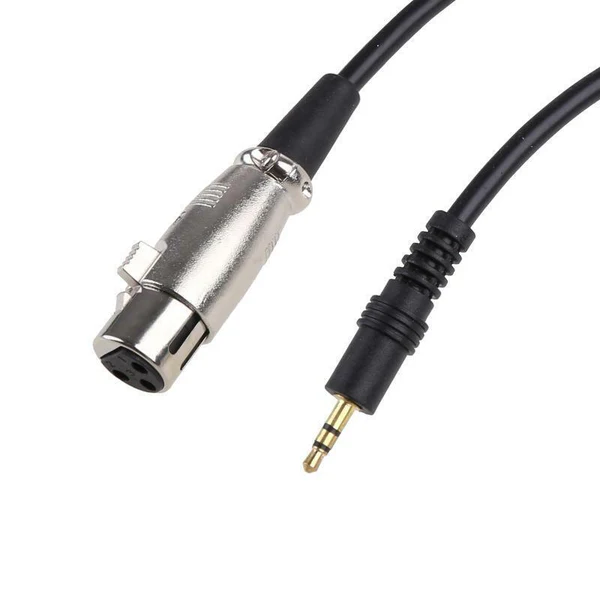
\includegraphics[width=0.25\textwidth]{images/xlr.png}
    \caption{Καλώδιο ήχου XLR δίπλα σε τυπικό 3.5 χιλιοστών καλώδιο ήχου}
  \end{figure}
\end{frame}

\begin{frame}[allowframebreaks]{Παρεμβολή}
  \begin{block}{3.5mm Jack (Unbalanced Signal)}
    Το καλώδιο 3.5mm jack μεταφέρει το σήμα μέσω ενός αγωγού, ενώ η γείωση χρησιμεύει ως αναφορά.
    Το σήμα με παρεμβολή περιγράφεται ως:
    \[
      V_{\text{output}} = V_{\text{signal}} + V_{\text{noise}}
    \]
    όπου:
    \[
      V_{\text{noise}}\footnote{Το αρχικό σήμα} \propto \frac{\Phi_{\text{EMI}}\footnote{Ο θόρυβος που προστίθεται στο σύστημα λόγω ηλεκτρομαγνητικών παρεμβολών}}{d}
    \]
    Μεγαλύτερα μήκη καλωδίων (\(d\)) οδηγούν σε περισσότερη παρεμβολή.
  \end{block}
  \begin{block}{XLR (Balanced Signal)}
    Το XLR χρησιμοποιεί δύο αγωγούς (\(+V\) και \(-V\)) που μεταφέρουν αντίθετα σήματα. Το σήμα με παρεμβολή περιγράφεται ως:
    \[
      V_{\text{output}} = (V_{\text{signal}} + V_{\text{noise}}) - (-V_{\text{signal}} + V_{\text{noise}})
    \]
    Αναπτύσσοντας:
    \[
      V_{\text{output}} = 2V_{\text{signal}}
    \]
  \end{block}
  \textbf{Σημείο-κλειδί:} Ο θόρυβος \(V_{\text{noise}}\) εξουδετερώνεται πλήρως\footnote{Βλέπε Common-Mode Rejection (CMR)}
  , ενώ το σήμα ενισχύεται.

  \begin{block}{Συμπερασματικά}
    \begin{itemize}
      \item \textbf{3.5mm Jack:} Το σήμα περιλαμβάνει θόρυβο:
            \[
              V_{\text{output}} = V_{\text{signal}} + V_{\text{noise}}
            \]
      \item \textbf{XLR:} Ο θόρυβος εξουδετερώνεται:
            \[
              V_{\text{output}} = 2V_{\text{signal}}
            \]
    \end{itemize}
  \end{block}
\end{frame}
\begin{frame}[allowframebreaks]{Κονσόλα ήχου}
  \begin{figure}
    \centering
    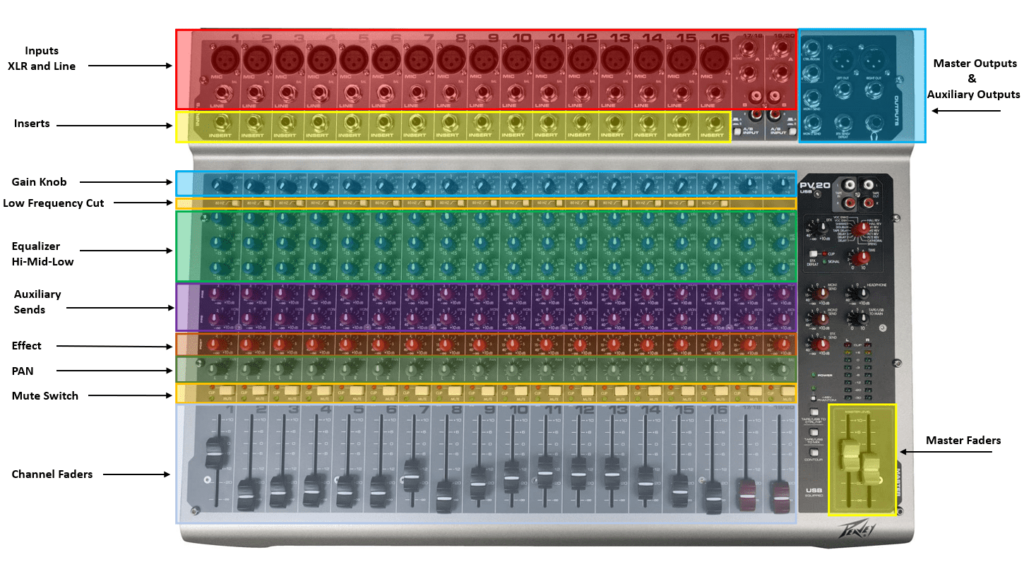
\includegraphics[width=0.6\textwidth]{images/mixer.png}
    \caption{Κονσόλα ήχου και τα βασικά της στοιχεία}
  \end{figure}

  \begin{block}{Οι ανάγκες μας;}
    \begin{itemize}
      \item τουλάχιστον 4 εισόδους (2 XLR και 2 3.5mm).
      \item Καλώδια XLR για τη σύνδεση μικροφώνων και των ηχείων.
      \item Τουλάχιστον 2 εξόδους XLR για τη σύνδεση των ηχείων.
      \item 48v phantom power για τη σύνδεση τυχών μικροφώνων (στην εγκατάσταση
            του αμφιθεάτρου κάτι τέτοιο δεν χρειάζεται).\footnote{Σκεφτείτε το phantom power ως το Power over ethernet των μικροφώνων}
    \end{itemize}
  \end{block}
\end{frame}
\begin{frame}[allowframebreaks]{Εικόνα και Βίντεο}

  \begin{itemize}
    \item HDMI Capture Card (π.χ., Elgato Camlink, Blackmagic\footnote{γνωστή κυρίως για το πρόγραμμα επεξεργασίας Video Davinci Resolve} Atem mini).
    \item Κάμερες και μικρόφωνα (τουλάχιστον 1080p ανάλυση).
  \end{itemize}
  \begin{block}{HDMI Capture Cards}
    \begin{figure}
      \centering
      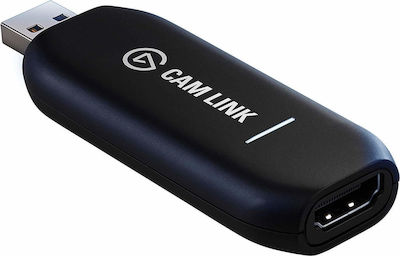
\includegraphics[width=0.15\textwidth]{images/elgato.jpeg}
      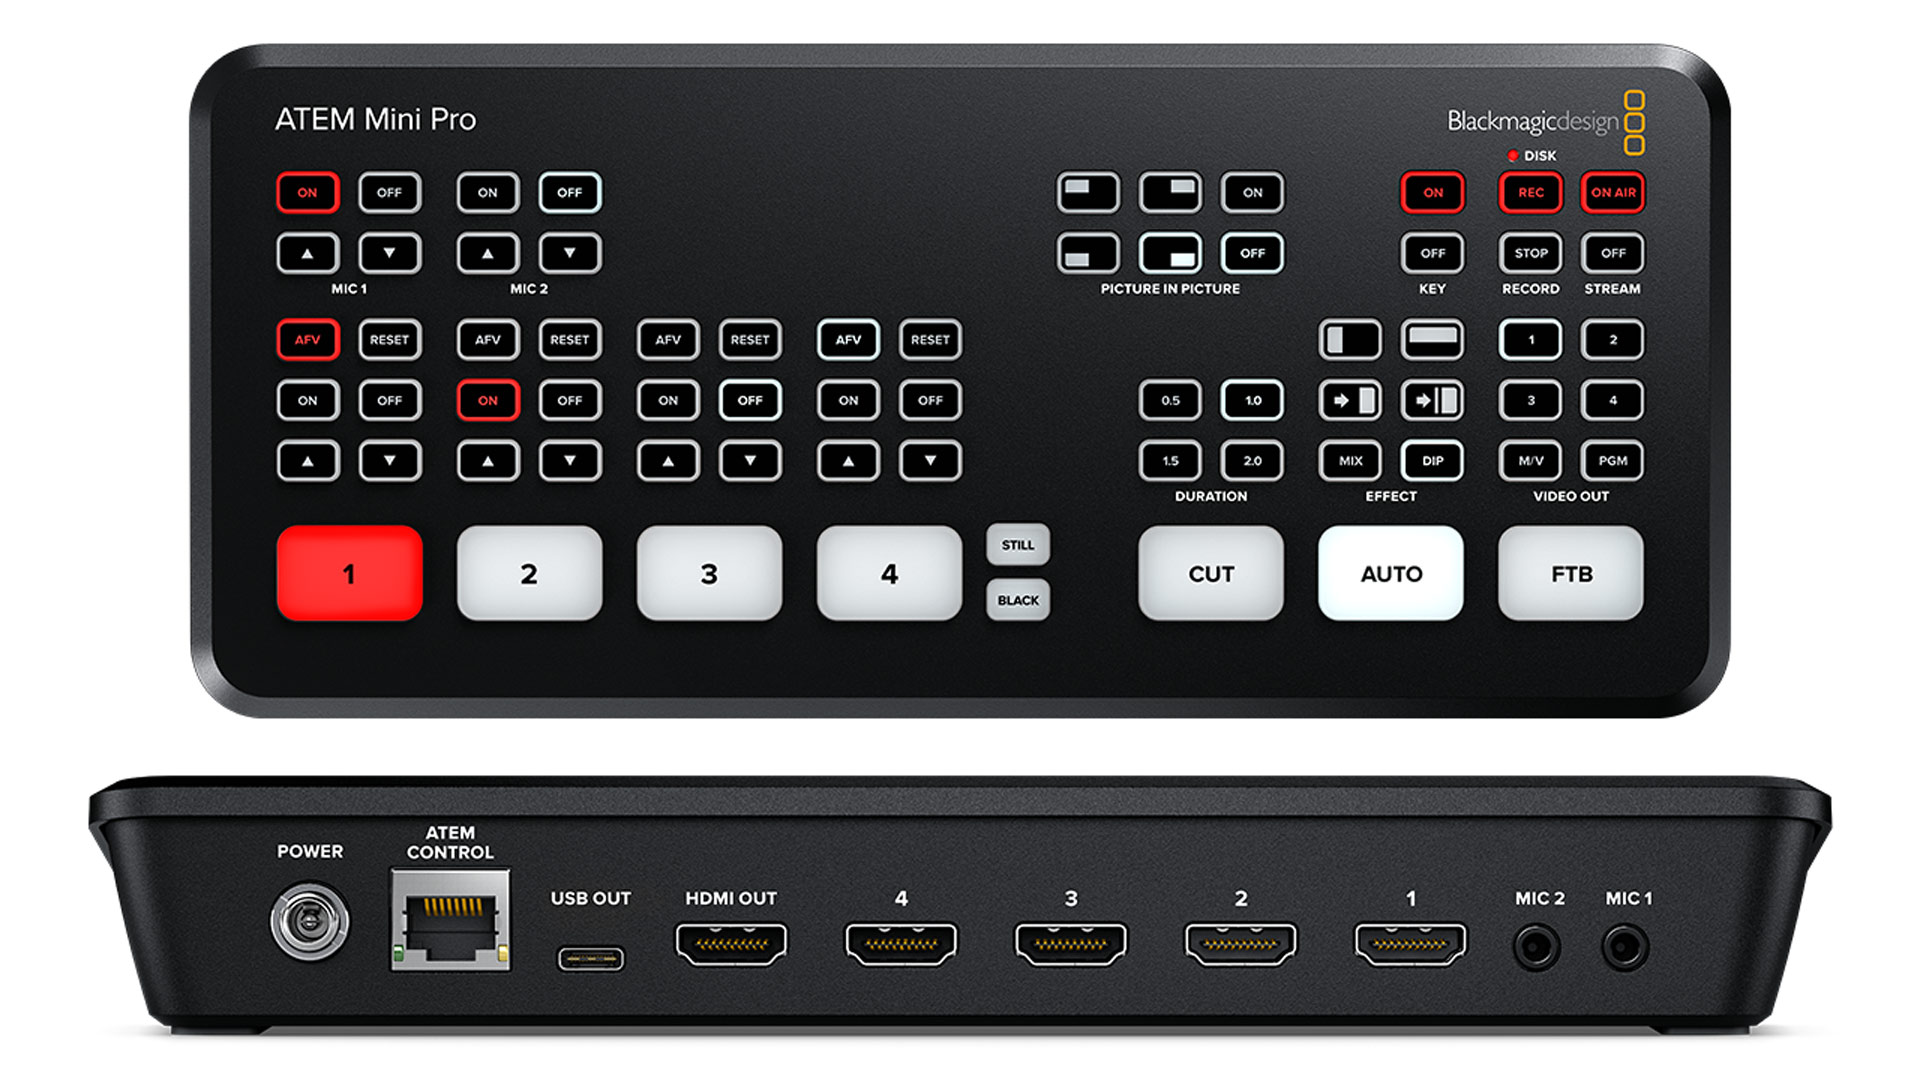
\includegraphics[width=0.25\textwidth]{images/atem.jpg}
      \caption{Elgato Camlink και κονσόλα καταγραφής audio/video Atem mini\footnote{Πιο ευέλικτη κάρτα καταγραφής από την Camlink, αλλά και πιο ακριβή}}
    \end{figure}
  \end{block}
  \begin{figure}
    \centering
    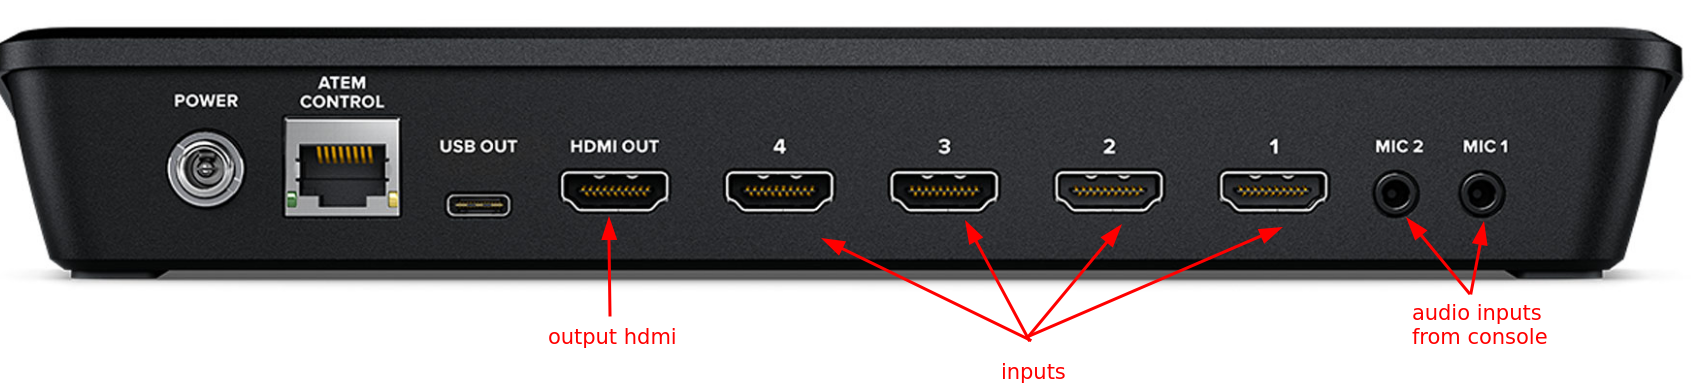
\includegraphics[width=0.8\textwidth]{images/atem_explanation.png}
    \caption{Ανάλυση των θυρών της κονσόλας Atem mini}
  \end{figure}
\end{frame}

\begin{frame}[allowframebreaks]{Ρυθμίσεις Εξοπλισμού}
  \begin{block}{Σχετικά με την κονσόλα ήχου}
    \begin{itemize}
      \item Ρύθμιση των επιπέδων εισόδου και εξόδου.
      \item Ενεργοποίηση του phantom power για τα μικρόφωνα.
      \item Ρύθμιση των επιπέδων εξόδου για τα ηχεία.
      \item Ενεργοποίηση του audio monitoring για τεχνικό έλεγχο
    \end{itemize}
  \end{block}
  \begin{exampleblock}{Χρησιμοποιόντας την έξοδο της κονσόλας ως μικρόφωνο}
    \begin{itemize}
      \item Χρήσιμη για παρακολούθηση ήχου.
      \item Ιδανική για τεχνικό έλεγχο.
      \item Χρήση της εξόδου της κονσόλας ως είσοδο μικροφώνου του υπολογιστή
            \begin{itemize}
              \item Έτσι ακούγεται η \enquote{αίθουσα} διαδικτυακά
              \item Αποφεύγουμε τον μικροφωνισμό\footnote{Θέλει πάντα προσεκτική σχεδίαση του συστήματός μας για να τον αποφύγουμε}
            \end{itemize}
    \end{itemize}
  \end{exampleblock}
  \begin{block}{One computer to rule them all}
    Απαιτήσεις:
    \begin{itemize}
      \item CPU: i5 ή ανώτερο.
      \item GPU: NVIDIA GTX 1660 ή νεότερη.
      \item RAM: 16GB+ \footnote{Σε Linux αρκούν και 8GB μνήμης}.
    \end{itemize}
    Ο κακός υπολογιστής είναι σαν να τρέχεις μαραθώνιο με σαγιονάρες. Απλά δεν γίνεται

  \end{block}
\end{frame}

\begin{frame}{Λογισμικό για Υβριδική Κάλυψη}
  \textbf{OBS (Open Broadcaster Software):}
  είναι ένα δωρεάν και ανοιχτού κώδικα λογισμικό που χρησιμοποιείται για
  εγγραφή και ζωντανή μετάδοση βίντεο και ήχου
  \begin{itemize}
    \item \textbf{Τι κάνει:}
          \begin{itemize}
            \item Εγγραφή και μετάδοση σε πραγματικό χρόνο.
            \item Ενσωμάτωση πηγών ήχου/βίντεο.
          \end{itemize}
    \item \textbf{Βασικές λειτουργίες:}
          \begin{itemize}
            \item Ρυθμίσεις απλών ή σύνθετων σκηνών (π.χ. Picture in Picture ή ειδικά εφέ).
            \item Ροή (streaming) σε Zoom, YouTube, Facebook.
            \item recording της ροής στον τοπικό υπολογιστή
          \end{itemize}
    \item Το OBS είναι ο Ελβετικός σουγιάς των μεταδόσεων
  \end{itemize}
\end{frame}
\begin{frame}{Διάγραμμα μιας τυπικής υβριδικής αναμετάδοσης}
  \begin{figure}
    \centering
    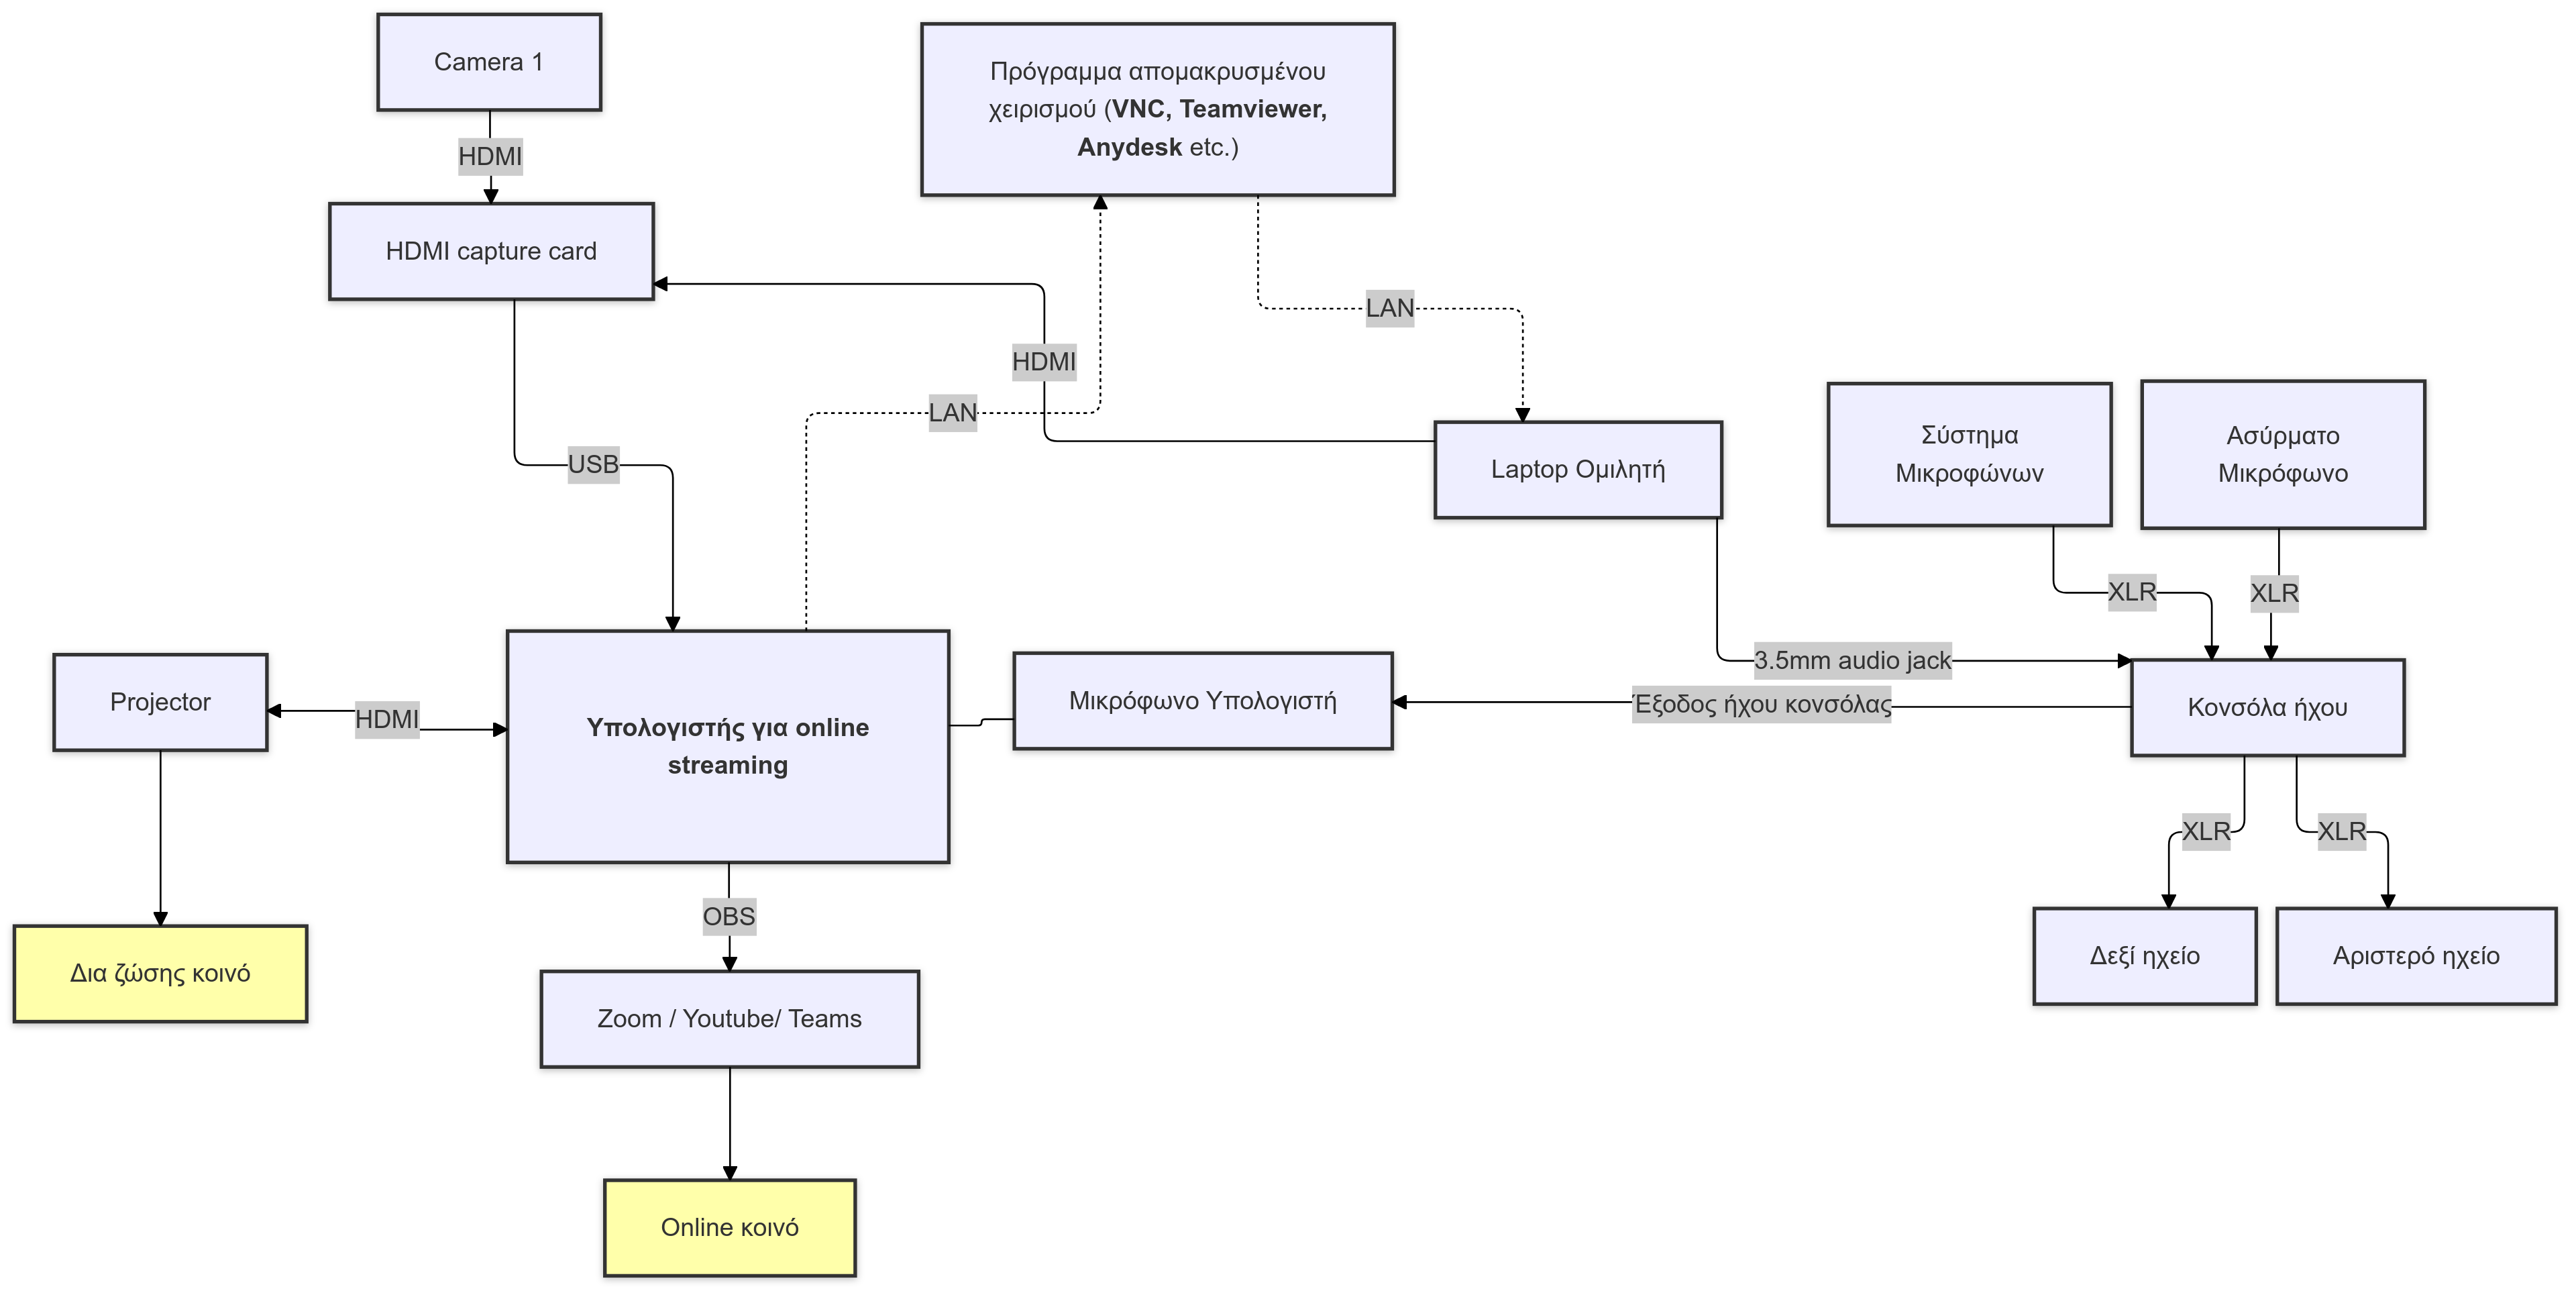
\includegraphics[width=0.8\textwidth]{images/diagram.png}
    \caption{Διάγραμμα ενός συστήματος υβριδικής αναμετάδοσης}
  \end{figure}
\end{frame}
\begin{frame}{Διάγραμμα του αμφιθεάτρου μας}
  \begin{figure}
    \centering
    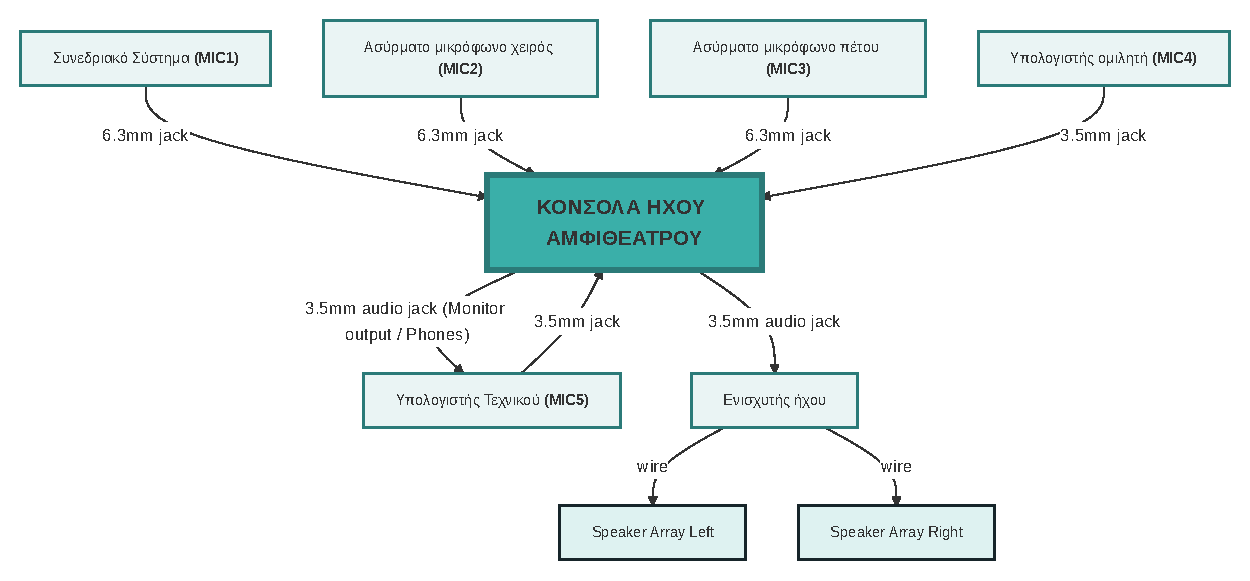
\includegraphics[width=0.8\textwidth]{images/amfitheatro.pdf}
    \caption{Διάγραμμα του ηχητικού συστήματος του αμφιθεάτρου μας}
  \end{figure}
\end{frame}
\begin{frame}{OBS και Zoom}
  \begin{block}{Πώς να μεταδώσεις απευθείας στο Zoom;}
    \begin{enumerate}
      \item Στήσε τη σκηνή σου στο πρόγραμμα OBS.
      \item Ρύθμισε το OBS Virtual Camera.
      \item Επέλεξε το OBS Virtual Camera ως πηγή βίντεο στο Zoom.
    \end{enumerate}
  \end{block}
  \begin{exampleblock}{Χρήσιμες συμβουλές}
    \begin{itemize}
      \item Ρύθμισε την εικόνα και τον ήχο πριν απο την.
      \item Έχε πάντα ένα backup σχέδιο.
      \item Έχε υπομονή και όρεξη.
      \item Ελέγξτε τη σύνδεση δικτύου (upload speed > 10Mbps).
      \item Ενεργοποιήστε την ανατροφοδότηση (audio monitoring) για έλεγχο.
    \end{itemize}
  \end{exampleblock}
\end{frame}

\section{Ανακεφαλαίωση}
\begin{frame}{Συμπερασματικά}
  \begin{itemize}
    \item Η υβριδική κάλυψη είναι η γέφυρα ανάμεσα στον ψηφιακό και φυσικό κόσμο των εκδηλώσεων.
    \item Με τον σωστό εξοπλισμό και προγραμματισμό, όλα είναι δυνατά.
    \item Και θυμηθείτε, αν κάτι πάει στραβά... πάντα φταίει το Internet!
  \end{itemize}
\end{frame}
\begin{frame}{Άδεια Χρήσης}
  \begin{center}
    \ccbysa
  \end{center}
  \begin{center}
    άδεια \href{https://creativecommons.org/licenses/by/4.0/}{Creative Commons Αναφορά Δημιουργού 4.0 Διεθνές (CC BY 4.0)}.  Το παρόν διατίθεται υπό την
    \ccbysa
  \end{center}
  \begin{exampleblock}{Επιτρέπεται στον αποδέκτη:}
    \begin{itemize}
      \item Να μοιραστεί το έργο με άλλους.
      \item Να τροποποιήσει το έργο για προσωπική ή εμπορική χρήση.
      \item Να χρησιμοποιήσει το έργο σε παρουσιάσεις ή δημοσιεύσεις.
      \item Να αναφέρει τον δημιουργό του έργου όταν το χρησιμοποιεί.

    \end{itemize}
  \end{exampleblock}
\end{frame}
\end{document}
